\scanpage{88}
\mspage{- 24 -}
\uline{Preuve} : Soit $G$ un faisceau $C'$-acyclique. Il suffit de montrer que pour tout objet $X$ de $C$,
\[
 \overset{\handwritten{\scriptscriptstyle\vee}}{H}{}^q(C^{\unsure{\wedge|\prime}}/X,\handwritten{\mathscr H}^{0}(u_s(G)))=0
 \qquad q\handwritten{>}0
\]

Il suffit donc de montrer que pour toute famille couvrante $\handwritten{\mathcal U}=(U_i\handwritten{\longrightarrow}X,\ i\handwritten{\in}I)$ dont l'existence est assurée par la condition (\unsure{CNC|CMC}), $H^q(\handwritten{\mathcal U},\handwritten{\mathscr H}^{0}(u_s(G)))=0\quad\handwritten{\forall}\ q\handwritten{>}0$. Mais $u$, étant un foncteur continu, transforme la famille couvrante $\handwritten{\mathcal U}$ en une famille couvrante de $u(X)$ ; et par définition du foncteur image directe, on a l'égalité :
\[
 H^q(\handwritten{\mathcal U},\handwritten{\mathscr H}^{0}(u_s(G))) =
 H^q(u(\handwritten{\mathcal U}),\handwritten{\mathscr H}^{0}(G))
\]
Le faisceau $G$ étant $C'$-acyclique, ces groupes sont nuls pour tout $q\handwritten{>}0$. \unsure{c\textsuperscript{o}q.f.d.|c.q.f.d.}

La notion de faisceau $C$-acyclique n'est pas intrinsèque. Elle ne dépend pas uniquement du topos $C^{\handwritten{\sim}}$ défini par le site $C$, mais aussi du site particulier choisi pour définir le topos $C^{\handwritten{\sim}}$ (3.11). Nous allons maintenant définir une propriété intrinsèque.

\margin{\handwritten{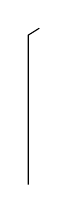
\begin{tikzpicture}[x=1em,y=1em]\draw (0.4,0.25)--(0,0)--(0,-5.4);\end{tikzpicture}}}
\uline{Proposition 3.4} : Soient $E$ un topos annelé par un anneau $A$ de $E$, $F$ un $A$-Module. Les propriétés suivantes sont équivalentes :

\unsure{i|1}) Pour tout objet $S$ de $E$ :
\[
 H^q(S,F)=0 \qquad \handwritten{\forall}\ q\handwritten{>}0\handwritten{.}
\]

\hfill .../...

% archive sheet number: 87
